\chapter{Variabili Aleatorie}

\begin{figure}[H]
    \centering
    \caption{Tipi di variabili casuali}
    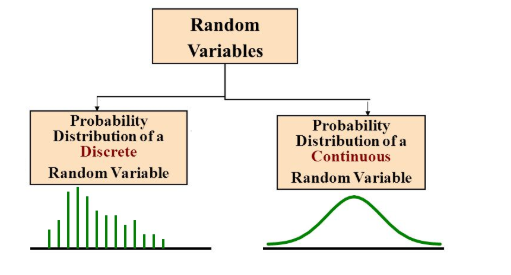
\includegraphics[]{varrandom}
\end{figure}

\section{Variabili Aleatorie Discrete}


Una variabile aleatoria \`e una funzione che pu\`o  assumere diversi valori in dipendenza da qualche fenomeno casuale.
Il risultato del lancio di un dado, o la vincita legata a tale risultato, ad esempio, sono variabili aleatorie.
\begin{defn}
    Prendiamo uno spazio probabilizzabile $ (\Omega, F) $. Una variabile aleatoria discreta \`e una funzione $ X : \Omega \to \R $, che assume valori in un sottoinsieme finito o numerabile
    $ \{a_1, \dots, a_k, \dots \} \subset \R$ e tale che 
    $ \forall j $ la controimmagine di $a_j$ sia un elemento della $\sigma$-algebra, ovvero che
    $$ X^{-1}(a_j) = \{ \omega \in \Omega, X(\omega) = a_j\} \in F. $$
\end{defn}

\begin{defn}
    Data la probabilit\`a  di tutti gli eventi posso definire la densit\`a  di probabilit\`a associata ad $X$: nello spazio probabilizzato $ (\Omega, F, P) $ la probabilit\`a  che la variabile aleatoria assuma il valore $ a_j $ sar\`a  $ p_j = \p{X = a_j} = \p{X^{-1}(a_j)} $. La successione $\{p_j\}$ viene detta {\em densit\`a  di probabilit\`a di $X$}.
\end{defn}
Dato che $X$ \`e una funzione valgono le seguenti propriet\`a

\begin{enumerate}
    \item $ \forall j$ gli insiemi $X^{-1} (a_j) $ sono tutti disgiunti.
    \item La loro unione copre $ \Omega $
\end{enumerate}
\begin{prop}
    La successione $\{p_j\}$ sopra definita  \`e  effettivamente una densit\`a  di probabilit\`a
\end{prop}
\begin{proof} Ovviamente abbiamo $p_j\ge0$ per ogni $j$. Inoltre vale $ \sum_{j=1}^{k} p_j = 1 $, infatti
    \begin{equation*}
        1 = \p{\Omega} = \p{\bigcup_{j} X^{-1}(a_j)} = \sum_{j} \p{X^{-1}(a_j)}
    \end{equation*}
\end{proof}
Sia $ X : \Omega \to \{ a_1, \dots, a_k ,\dots \} $ una variabile aleatoria definita su uno spazio probabilizzabile $ (\Omega, F) $, sia $\{p_j\}_j$ la densit\`a  di probabilit\`a di $X$. Allora si pu\`o dotare
$ (\Omega, F) $ della probabilit\`a indotta da $X$ definita come $ \p{X = a_j} = p_j $.

\begin{exmp}
    Preso uno spazio probabilizzabile $ (\Omega, F) $ e una variabile aleatoria $ X : \Omega \to \{ a_1, \dots, a_k \} $, supponendo che i numeri $ a_j $ siano ordinati, sia $ p_j $ la densit\`a  di probabilit\`a , come posso ricostruire, ad esempio $ \p{x \leq a_3} $?

    \begin{equation*}
        \p{X \leq a_3} = \p{X = a_1} + \p{X = a_2} + \p{X = a_3}=
        p_1+p_2+p_3
    \end{equation*}
\end{exmp}


\begin{exmp}
    Voglio contare quanti 6 escono in 10 lanci di dadi.
    
    Sia $ \Omega = \{ (1, 2, 3, 4, 5, 6)\}^{10} $, ovvero tutte le possibili parole di 10 elementi composte dai numeri da 1 a 6. Ad ogni lancio, ho $ \frac{1}{6} $ di probabilit\`a  di ottenere 6 e $ \frac{5}{6} $ di ottenere gli altri numeri. Definiamo la variabile aleatoria $ X : \Omega \to \{ 0, 1, 2, \dots, 9, 10 \} $ come il conteggio dei risultati dei lanci dove ottengo 6. Qual \`e la probabilit\`a  di ottenere 3 lanci dove ho fatto 6?
    Deve uscire 3 volte il numero 6, con probabilit\`a $1/6$, e 7 volte un numero diverso da 6,
    con probabilit\`a $5/6$. Inoltre non conta l'ordine, quindi devo moltiplicare per i modi in cui
    si prendono 3 oggetti (i tre dadi che hanno fatto 6) da un insieme di 10 elementi (tutti i lanci). 
    Abbiamo quindi
    \begin{equation*}
        \p{X = 3} = \binom{10}{3} \left(\dfrac{1}{6}\right)^3 \left(\dfrac{5}{6}\right)^7 
    \end{equation*}
\end{exmp}

\section{Variabili Aleatorie notevoli}

\begin{defn}
    \textbf{Legge di Bernoulli:}
    Faccio un esperimento, il risultato positivo ha probabilit\`a  $ p $, mentre il risultato negativo ha probabilit\`a  $ 1 - p $. Definisco $ \Omega = \{\text{successo},\text{insuccesso}\}$
    Una variabile aleatoria Bernoulliana \`e definita come
    \begin{eqnarray*}
    & X : \Omega \to \{0,1\}\\
    &X(\text{successo})=1 \\
    &X(\text{insuccesso})=0.
    \end{eqnarray*}
    Ovviamente avremo la densit\`a di $X$ data da $p_0=p$, $p_1=1-p$.
\end{defn}

\begin{defn}
    \textbf{Legge Binomiale}
    Sia $ k $ il conteggio dei successi di $ n $ esperimenti ripetuti, tutti indipendenti. Abbiamo quindi che $ B(n,p) : \Omega=\{\text{successo},\text{insuccesso}\}^n \to \{0, \dots, n\} $. Abbiamo che la densit\`a  di probabilit\`a  Binomiale $ p_k = \p{X=k} = \binom{n}{k} p^k(1-p)^{n-k} $ (abbiamo $k$ successi con prob. $p$,
 $n-k$ insuccessi di prob. $1-p$ e non conta l'ordine).
\end{defn}
Siamo sicuri che $ p_k $ sia una densit\`a ? Sappiamo che $ p_k \geq 0 $. Vediamo che $ 1 = \sum_{k} p_k $, infatti, ricordando che  $ (a+b)^n = \sum_{k=0}^{n} \binom{n}{k} a^k b^{n-k} $ (binomio di Newton), abbiamo che

\begin{equation*}
    \sum_{k} p_k = \sum_{k=0}^{n} \binom{n}{k} p^k (1-p)^{n-k} = (p+(1-p))^n = 1^n = 1
\end{equation*}

\begin{exmp}
    \textbf{Somma di Variabili Aleatorie}
    Lancio due dadi, uno rosso e uno nero, avremo quindi $ \Omega = \{(R, N)\ : \ R,N=1,\dots,6\}
    = \{(1,\dots,6)\}^2 $. Definisco due variabili aleatorie, $ X $ per il dado rosso dove $ X : (R, N) \to R $ e la variabile $ Y : (R, N) \to N $. La densit\`a  per $ X $ sar\`a  $ p_j = \frac{1}{6}$ $\forall j $ mentre la densit\`a  per $ Y $ sar\`a  $ q_j = \frac{1}{6}$ $\forall j $
    Definiamo $ Z = X + Y $ conta la somma dei dadi.



    Calcolare la densit\`a  di $ Z $

    In questo caso $ X, Y $ sono indipendenti, quindi avremo la densit\`a  di $ Z $ detta $ t_n $ con
    $n=2,\dots, 12$ data da
    
    \begin{equation*}
        t_n= \p{Z = n} = \sum_{i=1}^{n-1} \p{X = i} \cdot \p{Y = n - i}
    \end{equation*}
    
    \begin{table}[H]
        \centering
        \caption{Distribuzione discreta della somma del lancio di due dadi.}
        \label{tab:distribdice1}
        \begin{tabular}{|l|l|l|l|l|l|l|l|l|l|l|l|}
            \hline
            $ X + Y $     & 2        & 3        & 4        & 5        & 6        & 7        & 8        & 9        & 10       & 11       & 12       \\ \hline
            $ p_j + q_j $ & $ 1/36 $ & $ 2/36 $ & $ 3/36 $ & $ 4/36 $ & $ 5/36 $ & $ 6/36 $ & $ 5/36 $ & $ 4/36 $ & $ 3/36 $ & $ 2/36 $ & $ 1/36 $ \\ \hline
        \end{tabular}
    \end{table}
    
    \begin{figure}[H]
        \centering
        \caption{Distribuzione della somma del lancio di due dadi}
        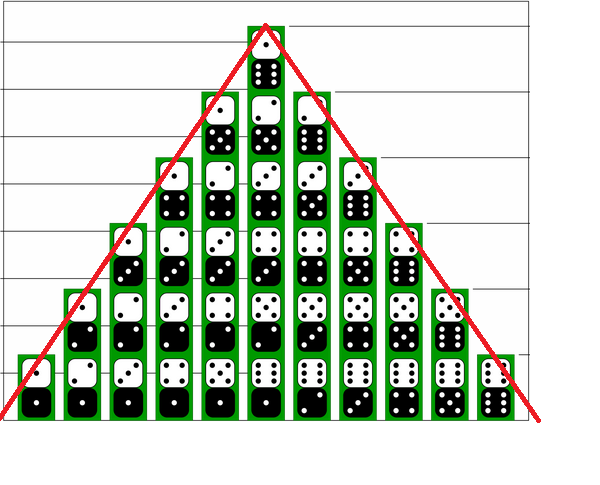
\includegraphics[]{binomdadi}
    \end{figure}
\end{exmp}

\begin{exmp}
    Calcolare $ \p{4 \leq Z \leq 6} $
    
    \begin{equation*}
    \p{4 \leq Z \leq 6} = \p{Z = 4} + \p{Z = 5} + \p{Z = 6} = \dfrac{3}{36} + \dfrac{4}{36} + \dfrac{5}{36} = \dfrac{12}{36} = \dfrac{1}{3}
    \end{equation*}
\end{exmp}		


\begin{defn}
    \textbf{Indipendenza di variabili aleatorie}
    Due variabili aleatorie $ X_1, X_2 $ sono indipendenti se $ \forall I_1, I_2, \subseteq \R $ intervalli o semirette si ha che 
    
    \begin{equation*}
        \left( \p{X_1 \in I_1} \cap \p{X_2 \in I_2} \right) = \p{X_1 \in I_1} \cdot \p{X_2 \in I_2}
    \end{equation*}
\end{defn}
    
    Nell'esempio di prima $ X, Z $  sono dipendenti perch\'e, dati $ I_1 = [3,4], I_2 = [1,2] $, allora si ha che $ \p{X\in I_1} = \p{X=3,4} = \dfrac{1}{3} $ e si ha anche $ \p{Z \in I_2} = \p{Z=1,2} = \p{Z=2} = \dfrac{1}{36} $. D'altra parte se ottengo 3 o 4 con il primo dado la somma sar\`a sempre superiore a 5, quindi

    \begin{equation*}
    \p{(X \in I_1) \cap (Z\in I_2)} =0\neq  \p{X \in I_1} \cdot \p{Z \in I_2}
    \end{equation*}



\begin{defn}
    \textbf{Variabili Aleatorie Congiunte}
    Due variabili aleatorie $ X,Y : \Omega \to \R $ discrete sono congiunte quando si pu\`o  calcolare $ \p{X = m \cap Y = n} = p_{n,m} $, ovvero una densit\`a  di probabilit\`a  $ \{ p_{n,m} \}_{n,m} $ con $ (p_{n,m} \geq 0 ) \land (\sum_{n,m} p_{n,m} = 1) $.
\end{defn}

Sapendo $ p_{n,m} $ ricavo tutti i $ \p{X=m} = p^X_m $ e $ \p{Y = n} = q^Y_n $ nel modo seguente

\begin{equation*}
    \begin{aligned}
    p^X_m =\p{X=m} = \p{X = m \cap \left\{ \bigcup_{n} Y=n \right\}} \\
    = \sum_{n} \p{X=m,Y=n} = \sum_n p_{n,m}\\
    q^Y_n=\p{Y=n} = \sum_{m} p_{n,m}
    \end{aligned}
\end{equation*}
    
In generale non si pu\`o  ricostruire dalle due densit\`a di probabilit\`a  la densit\`a della variabile aleatoria congiunta. Ad esempio, conoscendo $ p^X_n,q^Y_n $ cerco $ p_{n,m}  = \p{X = m \cap Y = n} = \p{X = m | Y = n} \cdot \p{Y=n} $, ma non conosco necessariamente $\p{X = m | Y = n}$
Se $ X,Y $ sono indipendenti allora $ P(X=m \mid Y=n) = \p{X=m} $ e vale il prodotto $ p_{m,n} = p^X_n \cdot q^Y_m $.
Si noti che in questo caso si verifica subito che  $ p_{m,n} $  \`e  una densit\`a  di probabilit\`a, infatti
$ p_{m,n}\ge0 $ perch\'e sia $p^X_n$  che $q^Y_m $ lo sono; inoltre

\begin{equation*}
    \sum_{m}\sum_{n} p_{n,m} = \sum_{m}\sum_{n} p^X_n \cdot q^Y_m
 = \left( \sum_{m} p^X_m \right) \left( \sum_{n} q^Y_m \right) = 1
\end{equation*}



\begin{defn}
    \textbf{Formula di Convoluzione}

    Tornando alla somma di due variabili aleatorie discrete, dati $ X,Y $ indipendenti e $ Z = X + Y $, con $ X,Y : \Omega \to \N $, se vogliamo calcolare $ \p{Z = n} $ e la densit\`a  di probabilit\`a  discreta $ \left\{Z = n\right\} $ possiamo usare le seguenti formule (dette di convoluzione)

    \begin{equation*}
    \begin{aligned}
    \left\{Z = n\right\} = \bigcup_{i=0}^{n} \left\{X = i \cap Y = n - i \right\} \\
    \p{z=n} = \sum_{i} \p{X = i \cap Y = n-i} = \sum_{i = n}^{n} \p{X=i} \cdot \p{Y=n-i}
    \end{aligned} 
    \end{equation*}
\end{defn}


Ho definito $ B(n,p)$ come i successi di $ n $ esperimenti che hanno successo con prob. $ p $.
In effetti vale la seguente formula
\begin{prop}
	Si ha che
	$B(n,p)= \sum_{i=1}^{n} \text{Bern}_i(p) $
\end{prop}
    \begin{proof}
        Caso base, per $ n = 1$ ovviamente $B(1,p) = \text{Bern}(p)$. Vediamo il passo induttivo:
        \begin{equation*}
        B(n,p) = \sum_{i=1}^{n} \text{Bern}_i(p) \implies B(n+1,p) = \sum_{i=1}^{n+1} \text{Bern}_i(p)
        \end{equation*}
        Quindi
        $$\sum_{i=1}^{n+1} \text{Bern}_i(p) = \left( \sum_{i=1}^{n} \text{Bern}_i(p) \right) + \text{Bern}_{n+1}(p) =
        B(n,p) + \text{Bern}(p)$$
        Introduciamo le densit\`a  per continuare la dimostrazione
        
        \begin{equation*}
        \begin{aligned}
        \p{B(n,p) + \text{Bern}(p) = k} = \p{B(n,p) = k \cap \text{Bern}(p) = 0} + \p{B(n,p) = k-1 \cap \text{Bern}(p) = 1} \\
        = \binom{n}{k-1}p^{k-1}(1-p)^{n-k+1} \cdot p + \binom{n}{k}p^k(1-p)^{n-k} \cdot  (1-p) \\
		= \left[\binom{n}{k-1}+\binom{n}{k}\right] p^k (1-p)^{n-k+1} = \binom{n+1}{k} p^k (1-p)^{n+1-k} = \p{B(n+1,p) = k}
        \end{aligned}
        \end{equation*}
    \end{proof}
    


\begin{defn}
    \textbf{Variabile Geometrica}
	Ripetiamo una successione esperimenti identici ed indipendenti con probabilit\`a  di successo $ 0 \leq p \leq 1 $  fino ad ottenere il primo successo. $ \geom(p) $ conta il numero di prove che abbiamo fatto. Ovvero $ \p{\geom(p) = k} = $ la probabilit\`a  di fare k esperimenti di cui i primi $k-1$ sono stati insuccessi e l'ultimo un successo. La densit\`a  di probabilit\`a  sar\`a quindi
	$$ p_k = \p{\geom(p) = k} = (1-p)^{k-1} \cdot p $$
\end{defn}
Ovviamente $ p_k \geq 0 $ e anche
$$ \sum_{k=1}^{\infty} (1-p)^{k-1} p = p \sum_{k=1}^{\infty}(1-p)^{k-1}= \dfrac{p}{1-(1-p)} = 1 $$ dalla somma della una serie geometrica. Quindi $p_k$ \`e una  densit\`a  di probabilit\`a

Una variabile geometrica \textbf{non ha memoria}, ovvero la probabilit\`a di avere un successo 
	 all'esperimento numero $ n $ dopo $n-1$ fallimenti ha la stessa probabilit\`a  avere un successo 
	 al primo esperimento. Infatti vale la seguente proposizione.
\begin{prop}	 
Si ha  
$$	\p{\geom(p) = n+m | \geom(p) > n} = \p{\geom(p) = m} $$
\end{prop}
\begin{proof}
    Notiamo che dire che abbiamo avuto successo alla prova $m+n$ gi\`a contiene l'informazione che abbiamo avuto almeno $n$ insuccessi. Inoltre $\geom(p) > n$ significa avere avuto sicuramente $n$ insuccessi, quindi
    $\p{\geom(p) > n}=(1-p)^n$, quindi si ha
    \begin{equation*}
        \begin{aligned}
            \p{\geom(p) = n+m \mid \geom(p) > n} =  \\
            = \dfrac{\p{\geom(p) = m + n \cap \geom(p) > n}}{\p{\geom(p) > n}} = \dfrac{\p{\geom(p) = m+n}}{\p{\geom(p) > n}}\\
            = \dfrac{(1-p)^{m+n-1} \cdot p}{(1-p)^n} = {(1-p)^{m-1} \cdot p}=\p{\geom(p) = m} \\
        \end{aligned}
    \end{equation*}
\end{proof}

    Si può dimostrare sapendo che $ \forall m . \p{\geom(p) = n+m \cap \p{\geom} > n} = \p{\geom(p) = m+n} $
    

\begin{defn}
    \textbf{Variabili Ipergeometriche}
    
	Siano dati $ r $ sfere rosse, $ b $ sfere bianche, $ n $ estrazioni senza reimbussolamento, $ k = $ numero di sfere rosse estratte, $ H(b+r, r, n) $ conta il numero di sfere rosse estratte dopo n tentativi. Questa variabile si chiama variabile ipergeometrica. Le condizioni di esistenza per i parametri sono $ (0 < n \leq b + r) \land (k \leq n)  \land (k \leq r) \land (n-k \leq b) $ ovvero $\max(0,n-b)\le k \le \min(n,r)$.

    Estrarre $k$ sfere rosse in $n$ estrazioni significa estrarne $k$ rosse e $n-k$ bianche, senza tener
	 conto dell'ordine, e i casi possibili sono $\binom{b+r}{n}$ (estrarre $n$ sfere da un totale di $b+r$)
	 Quindi la densit\`a  di probabilit\`a \`e
    \begin{equation*}
    \p{H(b+r, r, n) = k} = \dfrac{\binom{r}{k} \binom{b}{n-k}}{\binom{b+r}{n}}
    \end{equation*}
\end{defn}

\begin{exmp}
    Abbiamo 10 sfere rosse, 15 bianche e facciamo 7 estrazioni. Voglio contare il numero di sfere rosse estratte.

    Senza reimbussolamento: $H(25,10,7)$
    
    Con reimbussolamento: $B(7,2/5)$ (infatti sono 7 esperimenti identici con prob. di successo pari a
    $10/25=2/5$
\end{exmp}

\begin{defn}
    \textbf{Binomiale Negativa (o di Pascal)}
    Sia data una Bernoulliana di parametro $ p $. Ripetiamo l'esperimento fino a che non ho $ n $ successi. Quanti sono i fallimenti ottenuti?
	Se la binomiale negativa, indicata con $NB(n,p)$  ha valore $k$ significa che ho fatto $n+k$ prove,
	e ho avuto $ n $ successi e $ k $ fallimenti (in qualsiasi ordine)  la densit\`a di probabilit\`a  di una Binomiale Negativa quindi si definisce come

    \begin{equation*}
    \p{\nb{n, p} = k} = p^n(1-p)^k
    \end{equation*}
\end{defn}

Riassumendo: una variabile Binomiale conta i successi, una variabile Geometrica conta i fallimenti prima del primo successo e la Binomiale Negativa (NB) conta i fallimenti prima del successo $ n $-esimo. In una Binomiale Negativa non conta l'ordine degli esperimenti (tranne l'ultimo risultato). Le prove totali prima di avere $ n $ successi sono $ n+\text{NB} $.

\begin{exmp}
	Lancio una moneta fino ad ottenere 3 croci (non consecutive). Qual \`e la probabilit\`a  di aver fatto esattamente 2 risultati testa? E di avere ottenuto almeno una testa?

    $ \p{\nb{3, \frac{1}{2}} = 2} = \binom{3+2-1}{2} \left(\frac{1}{2}\right)^3 \left(\frac{1}{2}\right)^2 = \frac{3}{16} $.

	La probabilit\`a  di ottenere almeno un risultato testa \`e complementare ad avere ottenuto solo croci, quindi \`e pari a $1- \p{\nb{3, \frac{1}{2}} = 0} = 1 - \frac{1}{8} = \frac{7}{8} $
\end{exmp}

\section{Valore Atteso}

Consideriamo di voler calcolare la media pesata dei voti degli esami universitari. La media sar\`a  per ogni esame $ i $:
\begin{equation*}
    \sum_{i} \dfrac{(\text{voto})_i \cdot (\text{crediti})_i }{\sum_{i} \text{crediti}} = \sum_{i} (\text{voto})_i \cdot (\text{peso})_i
\end{equation*}
Se vogliamo definire la media, o il valore atteso di una variabile aleatoria discreta ragioniamo in
maniera analoga, con il $(\text{peso})_i$ sar\`a dato dalla probabilit\`a che $X$ assuma il valore $i$.
\begin{defn}
    \textbf{Media Pesata, Speranza o Valore Atteso}
	Sia $ X $ una variabile aleatoria discreta. La media di $ X $, detta anche \textbf{speranza} o \textbf{valore atteso} si definisce come
    \begin{equation*}
    \E{X} = \sum_{k} k \cdot \p{X = k} = \sum_{k} k \cdot p_k
    \end{equation*}

    Pi\`u in generale, data  $ f : \R \to \R $ per calcolare il valore atteso della variabile $f(X)$ si definisce

    \begin{equation*}
    \E{f(X)} = \sum_{k} f(k) \cdot p_k
    \end{equation*}
\end{defn}
\textbf{Osservazione} $\sum_{k} p_k = 1 $ \textbf{non implica che} $ \sum_{k} k p_k $ sia convergente. Se  $ \sum_{k} k p_k $ non converge ad un numero allora si dice che la variabile non ha media.
\begin{prop}
Se la variabile assume solo valori interi positivi allora

\begin{equation}\label{Ex}
\E{X} = \sum_{k=0}^\infty \p{X > k}
\end{equation}
\end{prop}
\begin{proof}
    Se si scrive $ \p{X > k} =  \p{X = k+1} + \p{X = k+2} + \dots $ per ogni $k$, e poi si inizia a sommare ci si accorge che $p_0$ non compare mai,
$p_1$ compare una sola volta, $p_2$ 2 volte e in generale $p_k$ compare esattamente $k$ volte.
Quindi  $\sum_{k} \p{X > k}\sum_{k} k p_k=\E{X} $.
\end{proof}

\begin{prop}
La speranza di una Binomiale $ B(n,p) $ vale $\E{B(n,p)}=np$ . 
\end{prop}
\begin{proof}
La densit\`a di $ B(n,p) $  \`e $ p_k = \binom{n}{k}p^k(1-p)^{n-k}$  $\forall k \in [0,n] $.
 Abbiamo che $ kp_k = k \binom{n}{k}p^k (1-p)^{n-k} = n \binom{n-1}{k-1} p^k(1-p)^{n-k} $. Definiamo $ h = k-1 $.

\begin{equation*}
    \begin{aligned}
        \E{B(n,p)} = \sum_{k=1}^{n} kp_k = \sum_{k=1}^{n} n \binom{n-1}{k-1} p^k(1-p)^{n-k} \\
        = np \sum_{k=1}^{n} \binom{n-1}{k-1}p^{k-1}(1-p)^{n-k} \\
        = np \sum_{h=0}^{n-1} \binom{n-1}{h} p^h(1-p)^{(n-1) - h } \\
        = np(p+(1-p))^{n-1} = np
    \end{aligned}
\end{equation*}
dove nell'ultimo passaggio abbiamo usato la formula del binomio di Newton.
\end{proof}

\begin{prop}
	La speranza di  di una variabile geometrica $ \geom(p) $ vale $\E{\geom(p)} =1/p$.
\end{prop}
\begin{proof}	
Usiamo la formula (\ref{Ex}), perch\'e altrimenti non \`e banale nemmeno dimostrare la convergenza della 
serie.
		\begin{equation*}
	\E{\geom(p)} = \sum_{k=0}^\infty\p{\geom(p) > k}
	\end{equation*}
	Come abbiamo gi\`a osservato $\p{\geom(p) > k}=(1-p)^k$, quindi
		\begin{equation*}
		\sum_{k=0}^\infty\p{\geom(p) > k} =\sum_{k=0}^\infty(1-p)^k = \dfrac{1}{1-(1-p)} = \dfrac{1}{p}
	\end{equation*}
\end{proof}

\begin{exmp}
    Scommetto. Pago 1 euro. Lancio 3 dadi e guadagno 1 euro ogni 6 che esce.
	Rappresento il guadagno con una variabile binomiale $ X = B(3,1/6) - 1$. Abbiamo che $ \E{X} = \E{B(3,1/6)} - 1 = 3 \cdot 1/6 - 1 = -1/2$ (quindi non mi conviene scommettere!)
\end{exmp}
        

\begin{defn}
    \textbf{Distribuzione di Poisson}
    Nel caso di una variabile binomiale conosco $ p $ e $ n $ (numero esperimenti).
    In una distribuzione di Poisson si conosce una media $ \mu $ di successi in un intervallo di osservazione $ \tau $, e si suppone che nell'intervallo di tempo si verifichino molte prove indipendenti
	tra di loro. In qualche senso (euristico) la variabile di Poisson di parametro $\mu$ rappresenta
	il limite di una binomiale $B(n,p)$ con $n\rightarrow \infty$. 
	In effetti supponiamo che nell'intervallo $ \tau $ avvengano $ n $ prove di parametro $p$ tutte indipendenti tra di loro. Se abbiamo in media $ \mu $ successi per intervallo $\tau$,
	se $n$ \`e molto grande si pu\`o supporre che $ \mu = \E{B(n,p)} = np$. Per definire la Poisson
    allora proviamo a fare il limite di una densit\`a binomiale.
    \begin{equation*}
    \begin{aligned}
        \lim_{n\rightarrow\infty}\p{B(n,p) = k} =\lim_{n\rightarrow\infty} \binom{n}{k}p^k(1-p)^{n-k}
        = \lim_{n\rightarrow\infty} \binom{n}{k} \left(\dfrac{\mu}{n}\right)^k \left(1- \dfrac{\mu}{n}\right)^{n-k}
        = \\
        =\lim_{n\rightarrow\infty}\dfrac{n!}{k!(n-k)!} \dfrac{1}{n^k} \dfrac{\mu^k}{\left(1-\dfrac{\mu}{n}\right)^k} \cdot \left(1-\dfrac{\mu}{n}\right)^n  =
        \lim_{n\rightarrow\infty}\dfrac{n(n-1)\dots (n-k+1)}{n^k k!} \dfrac{\mu^k}{\left(1-\dfrac{\mu}{n}\right)^k} \cdot \left(1-\dfrac{\mu}{n}\right)^n
        = \\
        =\lim_{n\rightarrow\infty} \dfrac{1 \cdot \left(1-\dfrac{1}{n} \right) \cdot \left(1-\dfrac{2}{n}\right) \cdot \dots \cdot \left(1- \dfrac{k-1}{n}\right)}{k!} \cdot \dfrac{\mu^k}{\left(1-\dfrac{\mu}{n}\right)^k} \cdot \left(1-\dfrac{\mu}{n}\right)^n =\\
        = \dfrac{\mu^k}{k!} e^{-\mu}
    \end{aligned}
    \end{equation*}

	Con questo ragionamento (non rigoroso!) possiamo definire
    \begin{equation}
    \p{\text{Poisson}(\mu) = k} = \dfrac{\mu^k}{k!} e^{-\mu}
    \end{equation}

\end{defn}

La variabile di Poisson in qualche senso ci dice quanto \`e la probabilit\`a che in un certo intervallo di
tempo ci si discosti dal valore medio che ci si aspetta in uno stesso intervallo di tempo.

\begin{exmp}
	Siamo nel secolo 1800, prendiamo l'esercito di Napoleone nel reparto della cavalleria. Ogni anno 12 cavalieri muoiono per incidente a cavallo. Voglio sapere la probabilit\`a  che nel 1861 siano morti 7 cavalieri.
    \begin{equation*}
    \p{\text{anno } 1861 | \text{sono morti 7 cavalieri}}
    \end{equation*}
    Utilizziamo la distribuzione di Poisson.
    
    \begin{equation*}
    \p{\text{Poisson}(12) = 7} = \dfrac{12^7}{7}e^{-12} \approx 0.04
    \end{equation*}
    
\end{exmp}

\begin{prop}
	\textbf{Linearit\`a  della media}
    
    Siano date $ X,Y $ variabili aleatorie, $ \alpha ,\beta \in \R $. Abbiamo che
    
    \begin{equation*}
    \E{\alpha X + \beta Y} = \alpha \E{X} + \beta \E{Y}
    \end{equation*}
\end{prop}


\begin{proof} Dimostriamo la propriet\`a nel caso $\alpha=\beta=1$. La dimostrazione
    nel caso generale \`e assolutamente analoga. 
    Supponiamo anche, per semplificare le notazioni, che $X,Y$ assumano valori naturali.
    Come al solito, chiamiamo $p_{i,j}=\p{X=i\cap Y=j}$, $p_i^X=\p{X=i}$ e $q_j^Y=\p{Y=j}$
            \begin{equation*}
            \begin{aligned}
            \E{X+Y} = \sum_{i,j} (i+j)p_{i,j} = \sum_{i,j} ip_{i,j} + \sum_{i,j} jp_{i,j} \\
            = \sum_i i \sum_j p_{i,j} + \sum_j j \sum_i p_{i,j} \\
            = \sum_i i p_i^X + \sum_j jq_j^Y = \E{X} + \E{Y}
            \end{aligned}
            \end{equation*}
\end{proof}

\begin{prop}
	\textbf{Valore atteso del prodotto}
	Siano date $ X,Y $ variabili aleatorie \textbf{indipendenti}. Allora
	$$\E{X \cdot Y} = \E{X} \cdot \E{Y}
	$$
\end{prop}
\begin{proof}
    Se $X$ e $Y$ sono indipendenti, allora abbiamo che $p_{i,j}= p_i^X\cdot q_j^Y$, quindi
        \begin{equation*}
        \begin{aligned}
        \E{X \cdot Y} = \sum_{i,j} i  j  \p{X = i \cap Y =j} \\
        = \sum_{i,j} i  j p_{i,j} = \sum_{i,j} ij p_i^X q_j^Y =  \sum_{i} i p_i^X \cdot \sum j q_j^Y
        = \E{X} \cdot \E{Y}
        \end{aligned}
        \end{equation*}
\end{proof}


\begin{defn}
	\textbf{Momenti di ordine superiore}

	Si definisce $\E{X^n}$ il momento di $X$ di ordine n.
	Dalla definizione di valore atteso sappiamo, ad esempio $ \E{X^2} = \sum_i i^2 p_i$.
Attenzione: per quanto detto sopra, e visto che $X$ non \`e indipendente da se stessa, in generale
$ \E{X^2} \neq \left(\E{X}\right)^2$.
\end{defn}


\begin{defn}
    \textbf{Varianza}
    
    Sia $ X $ una variabile aleatoria e $ \E{X} = \mu $ la sua media.
    La varianza di $ X $ si definisce come 
    
    \begin{equation*}
    \begin{aligned}
    \var{X} = \E{(X-\mu)^2} \\ 
    = \sum_i (i-\mu)^2 \p{X = i}
    \end{aligned}
    \end{equation*}
\end{defn}
\begin{prop}
    La varianza di $ X $ \`e anche $ \E{X^2} - \left(\E{X}\right)^2 $
\end{prop}
    \begin{proof}
        \begin{equation*}
        \begin{aligned}
        \sum_i (i-\mu)^2 p_i = \sum_i (i^2 -2i\mu + \mu^2) p_i \\
        = \sum_i i^2 p_i - 2\mu \sum_i i p_i + \mu^2 \sum_i p_i \\
        = \E{X^2} - 2\mu^2 + \mu^2 = \E{X^2} - \mu^2 \\
        = \E{X^2} - \left(\E{X}\right)^2 
        \end{aligned}
        \end{equation*}
    \end{proof}

Diamo ora alcune diseguaglianze utili (senza dimostrarle)



\begin{prop}
	\textbf{Disuguaglianza di H\"older}

    \begin{equation}
        \begin{aligned}
        \E{X \cdot Y} \leq (E[X^p])^{\frac{1}{p}} (E[Y^q])^{\frac{1}{q}} \\
        \text{con } \dfrac{1}{p} + \dfrac{1}{q} = 1
        \end{aligned}
    \end{equation}

    In particolare, per $p=q=2$,
    \begin{equation}
		\E{X \cdot Y} \leq \sqrt{E[X^2]E[Y^2]}
    \end{equation}

\end{prop}

\begin{prop}
    \textbf{Disuguaglianza di Markov}
	Sia $X \geq 0$ e $ a > 0$. Vale
    \begin{equation}
        \p{X > a} \le \dfrac{\E{X}}{a}
    \end{equation}
\end{prop}

\begin{prop}
	\textbf{Disuguaglianza di Chebishev}
	Sia $X \geq 0$ e $ a > 0$. Vale
	\begin{equation}
					\p{\abs{X - \mu} > a} \leq \dfrac{\var{X}}{a^2}
	\end{equation}
\end{prop}
Della disuguaglianza di Chebishev diamo anche la dimostrazione.
\begin{proof}
    \begin{equation*}
        \begin{aligned}
            \p{\abs{X - \mu} > a} = \sum_{n \text{ t.c.} \abs{n - \mu} > a} \p{X = n} \\				\text{se } \abs{n - \mu} > a \text{ allora } 1 \le \dfrac{\abs{n - \mu}^2}{a^2} \\
            \implies  \sum_{n \text{ t.c.} \abs{n - \mu} > a}  p_n
                \leq \sum_{n \text{ t.c.} \abs{n - \mu} > a}  \dfrac{\abs{n - \mu}^2}{a^2} p_n \leq \dfrac{1}{a^2} \sum_{n\in \N} \abs{n - \mu}^2 p_n =\dfrac{\var{X}}{a^2}
        \end{aligned}
    \end{equation*}
\end{proof}

La varianza quindi misura, in qualche senso, quanto una variabile aleatoria si scosti dalla sua media.

\begin{defn}
    \textbf{$\sigma$ Deviazione Standard}
    
    Sia $ X $ variabile aleatoria. Allora definiamo la deviazione standard $ \sigma(X) := \sqrt{\var{X}} $. 
\end{defn}
\begin{prop}
	Data $ \mu $ media di $ X $, e dati $ \alpha, \beta \in \R $ si ha allora che

	\begin{equation*}
		\begin{aligned}
			\var{\alpha X + \beta} = \alpha ^2 \var{X} \\
			 \sigma(\alpha X + \beta) =| \alpha| \sigma(X) 
					\end{aligned}
	\end{equation*}
\end{prop}
\begin{proof}
Dimostriamo solo la prima formula, la seconda segue immediatamente.
\begin{equation*}
		\begin{aligned}
	    	\var{\alpha X + \beta}
          = \E{(\alpha X + \beta)^2} - (\E{\alpha X + \beta})^2 \\
			= \E{\alpha^2 X^2 + 2 \alpha \beta X + \beta^2} - (\alpha \E{X} + \beta)^2 \\
			=\alpha^2 \E{ X^2} + 2 \alpha \beta  \E{ X} + \beta^2 -
			\alpha^2 (\E{X})^2 -2 \alpha \beta  \E{ X} - \beta^2 \\
			= \alpha^2 (\E{X^2} - (\E{X})^2) = \alpha^2 \var{X}
        \end{aligned}
	\end{equation*}


\end{proof}

\begin{defn}
    \textbf{Somma di varianza} 
    
    Siano date $ X,Y $ variabili aleatorie indipendenti $ \implies \var{X + Y} = \var{X} + \var{Y} $ 
    
    \begin{proof}
		\begin{equation*}
		\begin{aligned}
		\var{X+Y} = \E{(X+Y)^2} - (\E{X+Y})^2 \\
		= \E{X^2} - 2\E{X \cdot Y} + \E{Y^2}-(\E{X})^2 - 2\E{X}\E{Y} - (\E{Y})^2 \\
		= \var{X} + \var{Y} + 2(\E{XY} - \E{X}\E{Y})\\
		\end{aligned}
		\end{equation*}
    e se X,Y sono indipendenti si ha che	$2(E[XY] - \E{X}\E{Y}) = 0$
	\end{proof}
    
\end{defn}


\begin{exmp}
	Varianza di una Bernoulliana: $ X = B(1,p) $
	\begin{equation*}
	\begin{aligned}
		\E{X} = p \\
		\E{X}^2 = p^2 \\
		\var{X} = p-p^2 = p(1-p)
	\end{aligned}
	\end{equation*}
\end{exmp}

\begin{exmp}
	$ X = B(n,p) \implies \var{X} = nB(1,p) = np(1-p) $
\end{exmp}

\begin{exmp})
	$ X = \text{Poisson}(\lambda)  \implies  \var{\text{Poisson}(\lambda)} = \lambda $
	(senza dim)
\end{exmp}





\section{Esercizi}

\begin{exrc}
    Ho una scatola con 12 lampadine, 4 di esse sono fulminate. Ne prendo 2. La probabilit\`a  che siano entrambe funzionanti \`e $ \p{H(12, 4, 2) = 0} = \dfrac{\binom{4}{0}\binom{8}{2}}{\binom{12}{2}} $
\end{exrc}
\begin{exrc}
    Ho una moneta truccata. La probabilit\`a  che esca testa \`e $ P_t = 0.55 $ e la probabilit\`a  che esca croce \`e $ P_c = 0.45 $. Lancio la moneta dieci volte, qual \`e la probabilit\`a  che avvenga la sequenza testa-croce per la prima volta al lancio 9-10? Perch\'e ci\`o  sia possibile deve uscire una sequenza composta da $ 0 \leq h \leq 8 $ lanci ``croce" consecutivi e $ 9-h $ lanci  ``testa" consecutivi, in modo da ottenere una sequenza formata da $ C^hT^{9-h}C $. La probabilit\`a  \`e $ \p{C^hT^{9-h}C} = (0.45)^h \cdot (0.55)^{9-h} \cdot (0.45) = (0.45)^{h+1} \cdot (0.55)^{9-h}$. La probabilit\`a  dell'unione $ \bigcup_{h} $ delle stringhe sar\`a  $ P = \sum_{h=0}^8(0.45)^{h+1}(0.55)^{9-h}$. Provare a svolgere l'esercizio usando la  variabile geometrica. Provare a fare l'esercizio con una moneta equilibrata. Come si semplifica la formula?


\end{exrc}

\begin{exrc}
	Un ubriaco cammina in una strada in pendenza. Va in salita con probabilit\`a  $ \p{\text{salita}} = 1/4 $ oppure in discesa con probabilit\`a  $ \p{\text{discesa}} = 3/4 $. Ogni 10 secondi decide casualmente una direzione. Si muove lungo un asse $ X $ partendo dall'origine a velocit\`a  $ \dfrac{1m}{10s} $. Qual \`e la posizione pi\`u probabile dopo $ 1 $ minuto? Introduciamo una variabile $ X = $ la posizione dopo 1 minuto. L'ubriaco si sposter\`a  al massimo di 6 metri in salita o 6 metri in discesa, quindi $ X \in \{-6,\dots +6\} $. Introduciamo anche la variabile $ Y = $ il numero di volte che l'ubriaco cambia direzione verso la discesa. $ Y $ \`e una variabile binomiale Bernoulliana (conta il numero di ``successi" in 6 esperimenti ripetuti) $ \implies Y = B(6, 3/4) $. Abbiamo che $ X = -1 \cdot Y + 1(6-Y) = 6 - 2Y $. Per quanto detto

    \begin{equation*}
        P^Y_k = \p{B(6, 3/4) = k} = \binom{6}{k} \left(\dfrac{3}{4}\right)^k \left(\dfrac{1}{4}\right)^{6-k}
    \end{equation*}
    
    \begin{table}[H]
        \centering
		\caption{Distribuzione della variabile $ Y $}
        \label{tab:ubriaco}
        \begin{tabular}{|l|l|l|l|l|l|l|l|}
            \hline \xrowht[()]{10pt}
            k     & 0                 & 1                        & 2                            & 3                            & 4                            & 5                           & 6                   \\ \hline \xrowht[()]{30pt}
            $P_k$ & $ \dfrac{1}{4^6}$  & $ \dfrac{6\cdot 3}{4^6}$ & $ \dfrac{15 \cdot 3^2}{4^6}$ & $ \dfrac{20 \cdot 3^3}{4^6}$ & $ \dfrac{15 \cdot 3^4}{4^6}$ & $ \dfrac{6 \cdot 3^5}{4^6}$ & $ \dfrac{3^6}{4^6}$ \\ \hline
        \end{tabular}
    \end{table}
    Il valore pi\`u probabile per $Y$ \`e quindi 5, e di conseguenza il valore pi\`u probabile per $X$ sar\`a
	-4.
\end{exrc}

\begin{exmp}
    Prendo un seme di carte francesi $ \{ A, 2, \dots, 10, J, Q, K \} $
    L'asso ha valore 11. I numeri da 2 a 10 hanno lo stesso valore del numero, le figure hanno valore 10. Estraggo una carta. Definiamo una variabile aleatoria $ X = $ punteggio. $ X \in \{2,3,4,5,6,7,8,9,10,11\} $. Abbiamo che $ p_k = 0 \iff k< 2 \land k > 11 $. Abbiamo anche che $ p_k = 1/13 \iff k=2,\dots,11$ e $ p_k = 4/13 \iff k=10$
\end{exmp}	

% TODO per casa

\begin{exrc}
	\`E pi\`u probabile fare almeno un 6 lanciando 4 dadi o almeno una coppia di 6 lanciando 25 volte una coppia di dadi?
\end{exrc}

\begin{exrc}
	Siano date due slot machines apparentemente identiche $ A,B $. La probabilit\`a  di vincere sulla $ A $ \`e $\dfrac{1}{2}$. La probabilit\`a  di vincere sulla $ B $ \`e $ \dfrac{1}{4}$. Calcolare $ \p{\text{aver giocato su }A \mid \text{aver vinto}} $ [Sugg.: usare Bayes e fattorizzazione]
\end{exrc}

\begin{exrc}
    Data un urna contenente 2 palline bianche e 5 nere. Se la prima estrazione \`e una pallina bianca, essa viene rimossa. Se invece \`e una pallina nera, la rimettiamo dentro e aggiungiamo altre 2 nere. Calcolare $ \p{\text{seconda estrazione sia una pallina nera}} $
\end{exrc}

\begin{exrc}
    In Finlandia il 70\% delle ragazze sono Bionde, il 20\% sono Rosse, il 10\% sono More. Hanno gli occhi Scuri il 10\% delle Bionde, il 25\% delle Rosse e il 50\% delle More.
    Conosco una ragazza (via email, quindi non ho foto) che dice di avere gli occhi scuri. Con che probabilit\`a  \`e bionda?

    I dati che abbiamo sono quindi: $\p{B}=7/10$,  $\p{R}=1/5$,  $\p{M}=1/10$,
    $\p{S \mid B}=1/10$,  $\p{S \mid R}=1/4$,  $\p{S \mid M}=1/2$,

    Utilizzando la formula di Bayes e di Fattorizzazione calcoliamo
    \begin{equation*}
    \begin{aligned}
    \p{B \mid S} = \dfrac{\p{S \mid B} \cdot \p{B}}{\p{S}} \\
	= \dfrac{\p{S \mid B} \cdot \p{B}}{\p{S \mid B} \p{B} + \p{S \mid R} \p{R} + \p{S \mid M} \p{M}} \approx 0.41
    \end{aligned}
    \end{equation*}
\end{exrc}

\begin{exrc}
    Ho 3 carte colorate sulla faccia e sul dorso. Una carta con la faccia rossa e il retro nero si scrive $ \dfrac{R}{N} $. Le tre carte sono quindi $ \dfrac{R}{N}, \dfrac{R}{R}, \dfrac{N}{N} $.
	Una di queste tre carte  \`e  sul tavolo e la faccia visibile \`e Rossa. Calcolare $ \p{\text{Faccia coperta } = R} $. Indichiamo con $ V $ la faccia Visibile e con $ C $ quella coperta.

    \begin{equation*}
    \begin{aligned}
    \p{C = R \mid V = R} = \dfrac{\p{C = R \cap V = R}}{\p{V = R}} = \dfrac{1/3}{1/2} = \dfrac{2}{3}
    \end{aligned} 
    \end{equation*}
\end{exrc}



\begin{exrc}
	Siano dati due eventi $A,B \subset \Omega$. Abbiamo che $ \p{A} = \dfrac{3}{4} $ e abbiamo $ \p{B} = \dfrac{1}{3} $. Possono essere disgiunti? No. Perch\'e la probabilit\`a  della loro unione \`e maggiore di uno $ \p{A \cup B} = \p{A} + \p{B} = \dfrac{3}{4} + \dfrac{1}{3} $, che \`e $ > 1 $. Abbiamo che $ A \cup B \subset \Omega $, ma $ 1 = \p{\Omega} > \p{A \cup B} $.
    
    Si verifichi la disuguaglianza $ \dfrac{1}{12} \leq \p{A \cap B} \leq \dfrac{1}{3} $.

    Sappiamo che
    \begin{equation*}
    \begin{aligned}
        A \cap B \subseteq A \text{ e } A \cap B \subseteq B \\
        \implies (\p{A \cap B} \leq \p{A}) \text{ e } (\p{A \cap B} \leq \p{B})) \\
    \implies \p{A \cap B} \leq \min\{\p{A}, \p{B}\} \\
    \end{aligned} 
    \end{equation*}
    
	Quindi che $ \p{A \cap B} \leq \dfrac{1}{3} $. Verifichiamo ora la prima parte della disuguaglianza
	$A = (A \cap B) \cup (A \cap B^C) $ e gli insiemi $(A \cap B)$ e $(A \cap B^C) $ sono disgiunti.
	Inoltre $A \cap B^C\subset B^C$
    Quindi
    \begin{equation*}
    \begin{aligned}
    \p{A \cap B} = \p{A} - \p{A \cap B^C} \geq \p{A} - \p{B^C} \\
    = \p{A} - (1-\p{B})
    = \p{A} + \p{B} - 1 = \dfrac{1}{3} + \dfrac{3}{4} - 1 = \dfrac{1}{12}
    \end{aligned}
    \end{equation*}
\end{exrc} 
\begin{exrc}
    Siano $X$ e $Y$ variabili aleatorie congiunte $X,Y:\Omega \rightarrow \{0,1\}$.
    Sia $p_i,j$ la densit\`a di probabilit\`a della variabile congiunta, con
    Si ha $p_{0,0}=0,51$, $p_{1,0}=0,02$, $p_{1,1}=0,46$.
    \begin{enumerate}
    \item Si determini $p_{0,1}$ [R: $p_{0,1}=0,01$]
    \item Si trovino le densit\`a di $X$ e di $Y$  [R: $p_0^X=0,52,\ p_1^X=0,48$ e
    $q_0^X=0,53,\ q_1^X=0,47$]
    \item Si calcoli $\E{X}$ e $\E{Y}$  [R: $\E{X}=0,48$ e $\E{Y}=0,47$]
    \item Le due variabili sono indipendenti? [R: No, ad es. $p_{0,1}\neq p_0^X\cdot q_1^Y$]
    \item Si calcoli $\p{X=1\  |\ Y=1}$ [R: $\p{X=1\  |\ Y=1}=\p{Y=1\  |\ X=1}/\p{X=1}\simeq 0,95$]
    \end{enumerate}
    \end{exrc}
    
    \begin{exrc}
    Sia $X$ una Bernoulliana di parametro $1/2$ e sia $Y$ una variabile aleatoria a valori in $\{1,2,3\}$
    tale che  $\p{Y=1\  |\ X=0}=0,1$; $\p{Y=2\  |\ X=0}=0,4$; $\p{Y=3\  |\ X=0}=0,5$; $\p{Y=1\  |\ X=1}=0,5$; 
    $\p{Y=2\  |\ X=1}=0,4$; $\p{Y=3\  |\ X=1}=0,1$.
    \begin{enumerate}
    \item Trovare la distribuzione congiunta di $X,Y$ e la distribuzione di $Y$
    [R: $\p{Y=1\  ,\ X=0}=\p{Y=1\  |\ X=0}/\p{X=0}=0,05$ ecc.]
    \item Calcolare $\E{Y}$ e $\var{Y}$ [R: $\E{Y}=2$, $\var{Y}=0,6$]
    \item Calcolare $\E{X}$ e $\E{XY}$ [R: $\E{X}=0,5$, $\E{XY}=0,8$]
    \item Dire se $X$ e $Y$ sono indipendenti [R: No]
    \item Trovare la densit\`a di probabilit\`a di $Z=X/Y$ [R: $\p{Z=0}=0,5$; 
    $\p{Z=1}=0,25$; $\p{Z=1/2}=0,2$; $\p{Z=1/3}=0,05$]
    \end{enumerate}
    \end{exrc} \begin{exrc} Si lancia un dado a 4 facce, con valori $N=\{0,1,2,3\}$. Il risultato ci dice quante 
    volte dobbiamo lanciare una moneta. La variabile $k$ conta il numero totale di teste uscite.
    \begin{enumerate}
    \item Determinare $p_{N,k}$ [R: $p_{N,k}=0$ se $k>N$ (non posso avere pi\`u teste di quante 
    volte ho lanciato la moneta) e $p_{N,k}=\binom{N}{k} \frac{1}{2^{N+2}}$ se $k\le N$]
    \item Calcolare $\p{N=2 | k=3}$ e $\p{N=3 | k=1}$ [R: $\p{N=2 | k=3}=0$;
    $\p{N=3 | k=1}$=3/11]
    \end{enumerate}
    \end{exrc} 
    
    \begin{exrc} Siano $X:\Omega\rightarrow \{-1,0,1\}$ e $Y:\Omega\rightarrow \{0,1\}$
    variabili congiunte, con $p_{1,1}=p_{1,0}=p_{0,0}=p_{-1,1}=1/10$; $p_{0,1}=p_{-1,0}=3/10$.
    \begin{enumerate} 
    \item Trovare $p^X_i$ e $q^X_j$.
    \item Dire se $X$ e $Y$ sono indipendenti
    \item Trovare la distribuzione di $X^2$ ed di $XY$
    \item Trovare valor medio e varianza di $X$, $Y$, $X^2$, $XY$. 
    \end{enumerate}
\end{exrc}


\section{Esercitazione del 29/10/19}

Lezione tenuta da Maurizio Pratelli.

\begin{exrc}
    Ci sono 3 monete indistinguibili, delle quali due sono truccate.
    La probabilit\`a che esca testa \`e nell'ordine 1/4, 1/2 e 3/4.
    Si sceglie una moneta casuale, si lancia 5 volte e si ottiene testa 4 volte: qual'\`e la probabilit\`a di aver scelto la terza moneta?

    Utilizziamo la formula di Bayes. Definiamo le 3 monete $A_1, A_2, A_3$. Sappiamo anche che $ \p{A_1} = \p{A_2} = \p{A_3} = \frac{1}{3} $. Definiamo l'evento $ B $ come "\textit{esce 4 volte su 5 testa}".

    \begin{equation*}
        \begin{aligned}
            \p{A_3 \mid B} = \dfrac{\p{B \mid A_3}}{\p{B \mid A_1} + \p{B \mid A_2} + \p{B \mid A_3}} \\
            \p{B \mid A_1} = \binom{5}{4} \left(\dfrac{1}{4}\right)^4 \cdot \dfrac{3}{4}\\
            \p{B \mid A_2} = \binom{5}{4} \left(\dfrac{1}{2}\right)^5 \\
            \p{B \mid A_3} = \binom{5}{4} \left(\dfrac{3}{4}\right)^4 \cdot \dfrac{1}{4}\\
        \end{aligned}
    \end{equation*}
\end{exrc}

\begin{exrc}
    Si prende un giorno a caso in un anno non bisestile ed \`e un mercoledì: in quel mese ci sono esattamente 4 mercoledì. Qual'\`e la probabilit\`a che quel giorno sia di febbraio?

    Definiamo
    \begin{itemize}
        \item $ A_1 = $ "Mese di 28 giorni". $ \p{A_1} = \dfrac{1}{12} $
        \item $ A_2 = $ "Mese di 30 giorni". $ \p{A_2} = \dfrac{4}{12} $
        \item $ A_3 $ = "Mese di 31 giorni". $ \p{A_3} = \dfrac{7}{12} $
        \item $ B = $ in quele mese ci sono 4 mercoledì.
    \end{itemize}

    \begin{equation*}
        \begin{aligned}
            \p{A_1 \mid B} = \p{B \mid A_1} \dfrac{\p{A_1}}{\p{B}} \\
            = \dfrac{\p{B \mid A_1} \p{A_1}}{\p{B \mid A_1}\p{A_1} + \p{B \mid A_2}\p{A_2} + \p{B \mid A_3}\p{A_3}} \\
            \p{B \mid A_1} = 1 \text{ (a febbraio ci sono sicuramente 4 mercoledì)} \\
            \p{B \mid A_2} = 1 - \dfrac{2}{7} = \dfrac{5}{7}\\
            \p{B \mid A_3} = \dfrac{4}{7}
        \end{aligned}
    \end{equation*}
\end{exrc}


\begin{exrc}
    Si lancia un dado equilibrato finch\'e il numero 6 esce per 2 volte
    (non necessariamente consecutive). Qual'\`e la probabilit\`a che anche il
    penultimo lancio fosse un 6?

    Sappiamo la definizione di variabile geometrica (conta il numero)
    di esperimenti con probabilit\`a $ p $ falliti necessari prima di ottenere un
    successo: $ X = \geom{p} $.

    \begin{equation*}
        \p{X = k} = (1-p)^{k-1}p \>\> \forall k
    \end{equation*}

    Definiamo $ Y = $ tentativi fino al secondo successo. I valori possibili sono 2, 3, 4...


    \begin{note}
        Serie geometriche da ricordare

        \begin{equation*}
            \begin{aligned}
                \abs{a} < 1 \implies \sum_{h=0}^{\infty} a^h = \dfrac{1}{1-a} \\
                \sum_{n=0}^\infty \dfrac{x^n}{n!} = e^x
            \end{aligned}
        \end{equation*}
    \end{note}

    Risolviamo l'esercizio.

    \begin{equation*}
        \begin{aligned}
            \p{Y = k} = (k-1)(1-p)^{k-1}\cdot p^2 \\
            \p{\text{Avere due successi consecutivi e prima nessuno}} \\
            = \sum_{k=2}^\infty (1-p)^{k-1}p^2 =  p^2 \sum_{h=0}^{\infty} (1-p)^h \\
            = \dfrac{p^2}{1-(1-p)} = p = \dfrac{1}{6}
        \end{aligned}
    \end{equation*}
\end{exrc}


\begin{exrc}
    Data una variabile aleatoria $ X $ per la quale si ha $ \E{X} = 1, \var{X} = 2$ e si ha che $ \E{X^4} = 10 $. Quanto vale la varianza di $ X $?

    \begin{equation*}
        \begin{aligned}
            \var{X} = \E{X^2} - \left( \E{X}^2 \right) \\
            \E{X^2} = 2 + 1^2 = 3 \\
            \var{X^2} = \E{X^4} - \left( \E{X^2} \right)^2 = 1
        \end{aligned}
    \end{equation*}
\end{exrc}

\begin{exrc}
    Si lancia per 15 volte un dado equilibrato e indichiamo con $ X $ la somma dei numeri ottenuti. Quanto vale \(\E{X}\)? Qual'\`e la varianza di \(X\)?

    \begin{equation*}
    \begin{aligned}
        X = X_1 + X_2 + \hdots + X_{15} \\
        X \text{ ha valori possibili } \left\{ 15, 16, 17, \hdots, 90\right\} \\
        \E{X} = \E{X_1} + \hdots + \E{X_{15}} = 15 \E{X_1} \\
        \var{X} = 15 \cdot \var{X_1} \\
        \E{X_1} = \dfrac{1 + 2 + 3 + 4 + 5 + 6}{6} = \dfrac{7}{2} \\
        \E{X_1^2} = \dfrac{\sum_{k=1}^6 k^2}{6} = \dfrac{91}{6}
    \end{aligned}
    \end{equation*}
\end{exrc}

\begin{exrc} (Roulette Russa)
    Paolo, Andrea e Giacomo sparano a turno in questo ordine con una pistola a tamburo a 6 colpi, nella quale \`e presente un solo proiettile, finch\'e il colpo non viene esploso. Si considerino queste due modalit\`a:
    \begin{itemize}
        \item a) il tamburo viene ruotato una volta sola all'inizio
        \item b) il tamburo viene ruotato prima di ogni colpo
    \end{itemize}

    Quale delle due modalit\`a \`e pi\`u conveniente per Giacomo, e quando e quanto \`e vantaggioso poter sparare per primo?

    Ogni giocatore ha \(1/3\) di probabilit\`a di vincere. Consideriamo il caso \textit{b}.

    \begin{equation*}
        \begin{aligned}
            \p{\text{vince Paolo}} = \frac{1}{6} + \left( \frac{5}{6} \right)^3 \cdot \frac{1}{6} + \left( \frac{5}{6} \right)^6 \cdot \frac{1}{6} + \hdots = \frac{1}{6} \\
            = \frac{1}{6} \cdot \sum_{h=0}^\infty \left( \left( \frac{5}{3} \right)^2 \right)^h = \frac{1}{6} \cdot \frac{1}{1- \frac{5^3}{6^3} } = \frac{36}{216 - 125} = a \\ \\
            \p{\text{vince Andrea}} = \frac{5}{6} \cdot \frac{1}{6} + \left( \frac{5}{6} \right)^4 \cdot \frac{1}{6} = \frac{5}{6}a \\ \\
            \p{\text{vince Giacomo}} = \left( \frac{5}{6} \right)^2 a
        \end{aligned}
    \end{equation*}

    % TODO sistema
\end{exrc}


\begin{exrc}
    Un candidato affronta una test a risposte multiple, con 5 domande. Ogni domanda ha 4 risposte delle quali una sola \`e esatta: ogni risposta esatta \`e valutata un punto e ogni risposta errata \`e penalizzata con \(-1/4\). Consideriamo un candidato del tutto impreparato che risponde a caso. Quale punteggio ottiene in media? Qual'\`e la probabilit\`a di ottenere un punteggio di 2.5

    \begin{equation*}
        \begin{aligned}
            X = \text{risposte esatte} = \text{B}\left(5,\frac{1}{4}\right) \\
            Y = \text{punteggio} = X - \frac{1}{4} (5-x) = \frac{5}{4}X - \frac{5}{4} \\
            \text{Media del punteggio} \\
            \E{Y} = \frac{5}{4} \cdot \E{X} - \frac{5}{4} = \frac{5}{4} \cdot \frac{5}{4} - \frac{5}{4} = \frac{5}{16} \\
        \end{aligned}
    \end{equation*}

    Risolviamo il secondo punto. La probabilit\`a di ottenere un punteggio di 2.5.

    \begin{equation*}
        \begin{aligned}
            Y = 2.5 \\
            \frac{5}{4}X - \frac{5}{4} = 2.5 \\
            \p{Y = 2.5} = \p{X = 3} = \binom{5}{3} \cdot \left( \frac{1}{4} \right)^3 \cdot \left( \frac{3}{4} \right)^2
        \end{aligned}
    \end{equation*}

\end{exrc}